\documentclass[class=memoir, tikz, dvipsnames, extrafontsizes, 36pt,
	convert={convertexe={magick convert}, density=600,size=1056x1056,outext=.png, command=\unexpanded{%
      \convertexe\space
      -background\space none\space
      -density \density\space
      -trim \space
      \infile\space
      -resize \size\space
      -gravity \space center\space
      -extent \space\size\space
      -colorspace \space gray \space -auto-level \space -threshold \space 50\percent\space
%      -fuzz \space 20\percent\space
      -transparent \space black \space
      -shave \space 16x16\space
%      -scale \size\space
      Alt\\f10.png %\outfile
    }}
]{standalone}
%\documentclass[class=memoir, 36pt, extrafontsizes, dvipsnames, tikz]{standalone}
\usepackage{fontspec}
\setmainfont[Mapping=tex-text-ms]{EotE Symbol}
%\usepackage[dvipsnames]{xcolor}
\usepackage{tikz}
\usetikzlibrary{shapes, calc, positioning, knots, backgrounds}

\newcommand{\adv}{\scalebox{0.9}{a}}
\newcommand{\light}{\scalebox{0.9}{Z}}

%Set Margins
\setlength{\topmargin}{0cm}
\setlength{\headheight}{0pt}
\setlength{\textheight}{27.5cm}
\setlength{\oddsidemargin}{0cm}
\setlength{\evensidemargin}{0cm}
\setlength{\textwidth}{18.9cm}
\setlength{\parindent}{0pt}

\definecolor{boost}{RGB}{144,255,255}
\definecolor{blackish}{RGB}{10,10,10}
\definecolor{ability}{RGB}{128,128,255}
\definecolor{difficulty}{RGB}{64,0,128}
\definecolor{challenge}{RGB}{192,0,0}
\newlength{\dimensions}
\setlength{\dimensions}{1.5cm}

\begin{document}
%\begin{tikzpicture}[x=\dimensions, y=\dimensions]%b3
%\draw[draw=none, fill=black] (0,0) rectangle (1, 1);
%\draw[draw=none, color=white] (0, 0) rectangle node[midway] {s} (1, 1);
%\end{tikzpicture}

%\begin{tikzpicture}[x=\dimensions, y=\dimensions]%b4
%\draw[draw=none, fill=black] (-1,1) rectangle (1,-1);
%\draw[draw=none, color=white] (0.1, -0.1) rectangle node[midway] {s} (-0.9, 0.9);
%\draw[draw=none, color=white] (-0.1, 0.1) rectangle node[midway] {\adv} (0.9, -0.9);
%\end{tikzpicture}

%\begin{tikzpicture}[x=\dimensions, y=\dimensions]%b5
%\draw[draw=none, fill=black] (-1,1) rectangle (1,-1);
%\draw[draw=none, color=white] (0.1, -0.1) rectangle node[midway] {\adv} (-0.9, 0.9);
%\draw[draw=none, color=white] (-0.1, 0.1) rectangle node[midway] {\adv} (0.9, -0.9);
%\end{tikzpicture}

%\begin{tikzpicture}[x=\dimensions, y=\dimensions]%b6
%\draw[draw=none, fill=black] (0,0) rectangle (1, 1);
%\draw[draw=none, color=white] (0, 0) rectangle node[midway] {\adv} (1, 1);
%\end{tikzpicture}

%\begin{tikzpicture}[x=\dimensions, y=\dimensions]%s3
%\draw[draw=none, fill=black] (0,0) rectangle (1, 1);
%\draw[draw=none, color=white] (0, 0) rectangle node[midway] {f} (1, 1);
%\end{tikzpicture}

%\begin{tikzpicture}[x=\dimensions, y=\dimensions]%s5
%\draw[draw=none, fill=black] (0,0) rectangle (1, 1);
%\draw[draw=none, color=white] (0, 0) rectangle node[midway] {t} (1, 1);
%\end{tikzpicture}

%\begin{tikzpicture}[x=1.1\dimensions, y=1.1\dimensions]%a2
%\draw[draw=none, fill=black] (-1,-1) rectangle (1, 1);
%\node[color=white] at (0,0) {s};
%\end{tikzpicture}

%\begin{tikzpicture}[x=1.1\dimensions, y=1.1\dimensions]%a5
%\draw[draw=none, fill=black] (-1,-1) rectangle (1, 1);
%\node[color=white, rotate=180] at (0,0) {\adv};
%\end{tikzpicture}

%\begin{tikzpicture}[x=1.1\dimensions, y=1.1\dimensions]%a4
%\draw[draw=none, fill=black] (-1,-1) rectangle (1, 1);
%\node[color=white] at (0,-0.15) {\scriptsize s};
%\node[color=white] at (0,0.35) {\scriptsize s};
%\end{tikzpicture}

%\begin{tikzpicture}[x=1.1\dimensions, y=1.1\dimensions]%a7
%\draw[draw=none, fill=black] (-1,-1) rectangle (1, 1);
%\node[color=white, rotate=180] at (0,-0.15) {\scriptsize \adv};
%\node[color=white] at (0,0.35) {\scriptsize s};
%\end{tikzpicture}

%\begin{tikzpicture}[x=1.1\dimensions, y=1.1\dimensions]%a8
%\draw[draw=none, fill=black] (-1,-1) rectangle (1, 1);
%\node[color=white, rotate=180] at (0,-0.15) {\scriptsize \adv};
%\node[color=white, rotate=180] at (0,0.35) {\scriptsize \adv};
%\end{tikzpicture}

%\begin{tikzpicture}[x=1.1\dimensions, y=1.1\dimensions]%d2
%\draw[draw=none, fill=black] (-1,-1) rectangle (1, 1);
%\node[color=white, rotate=180] at (0,0) {f};
%\end{tikzpicture}

%\begin{tikzpicture}[x=1.1\dimensions, y=1.1\dimensions]%d3
%\draw[draw=none, fill=black] (-1,-1) rectangle (1, 1);
%\node[color=white, rotate=180] at (0,-0.15) {\scriptsize f};
%\node[color=white, rotate=180] at (0,0.35) {\scriptsize f};
%\end{tikzpicture}

%\begin{tikzpicture}[x=1.1\dimensions, y=1.1\dimensions]%d4
%\draw[draw=none, fill=black] (-1,-1) rectangle (1, 1);
%\node[color=white] at (0,0) {t};
%\end{tikzpicture}

%\begin{tikzpicture}[x=1.1\dimensions, y=1.1\dimensions]%d7
%\draw[draw=none, fill=black] (-1,-1) rectangle (1, 1);
%\node[color=white] at (0,-0.15) {\scriptsize t};
%\node[color=white] at (0,0.35) {\scriptsize t};
%\end{tikzpicture}

%\begin{tikzpicture}[x=1.1\dimensions, y=1.1\dimensions]%d8
%\draw[draw=none, fill=black] (-1,-1) rectangle (1, 1);
%\node[color=white] at (0,-0.15) {\scriptsize t};
%\node[color=white, rotate=180] at (0,0.35) {\scriptsize f};
%\end{tikzpicture}

%\begin{tikzpicture}[x=1.1\dimensions, y=1.1\dimensions]%p4
%\draw[draw=none, fill=black] (-1,-1) rectangle (1, 1);
%\node[color=white] at (0,-0.225) {\scriptsize s};
%\node[color=white] at (0,0.275) {\scriptsize s};
%\end{tikzpicture}

%\begin{tikzpicture}[x=1.1\dimensions, y=1.1\dimensions]%p7
%\draw[draw=none, fill=black] (-1,-1) rectangle (1, 1);
%\node[color=white, rotate=180] at (0,-0.225) {\scriptsize \adv};
%\node[color=white] at (0,0.275) {\scriptsize s};
%\end{tikzpicture}

%\begin{tikzpicture}[x=1.1\dimensions, y=1.1\dimensions]%p10
%\draw[draw=none, fill=black] (-1,-1) rectangle (1, 1);
%\node[color=white, rotate=180] at (0,-0.225) {\scriptsize \adv};
%\node[color=white, rotate=180] at (0,0.275) {\scriptsize \adv};
%\end{tikzpicture}

%\begin{tikzpicture}[x=1.1\dimensions, y=1.1\dimensions]%p12
%\draw[draw=none, fill=black] (-1,-1) rectangle (1, 1);
%\node[color=white] at (0,0) {x};
%\end{tikzpicture}

%\begin{tikzpicture}[x=1.1\dimensions, y=1.1\dimensions]%c2
%\draw[draw=none, fill=black] (-1,-1) rectangle (1, 1);
%\node[color=white, rotate=180] at (0,0.1) {f};
%\end{tikzpicture}

%\begin{tikzpicture}[x=1.1\dimensions, y=1.1\dimensions]%c4
%\draw[draw=none, fill=black] (-1,-1) rectangle (1, 1);
%\node[color=white, rotate=180] at (0,-0.2) {\scriptsize f};
%\node[color=white, rotate=180] at (0,0.3) {\scriptsize f};
%\end{tikzpicture}

%\begin{tikzpicture}[x=1.1\dimensions, y=1.1\dimensions]%c6
%\draw[draw=none, fill=black] (-1,-1) rectangle (1, 1);
%\node[color=white] at (0,0) {t};
%\end{tikzpicture}

%\begin{tikzpicture}[x=1.1\dimensions, y=1.1\dimensions]%c8
%\draw[draw=none, fill=black] (-1,-1) rectangle (1, 1);
%\node[color=white] at (0,-0.195) {\scriptsize t};
%\node[color=white, rotate=180] at (0,0.3) {\scriptsize f};
%\end{tikzpicture}

%\begin{tikzpicture}[x=1.1\dimensions, y=1.1\dimensions]%c10
%\draw[draw=none, fill=black] (-1,-1) rectangle (1, 1);
%\node[color=white] at (0,-0.21) {\scriptsize t};
%\node[color=white] at (0,0.29) {\scriptsize t};
%\end{tikzpicture}

%\begin{tikzpicture}[x=1.1\dimensions, y=1.1\dimensions]%c12
%\draw[draw=none, fill=black] (-1,-1) rectangle (1, 1);
%\node[color=white, rotate=180] at (0,0.055) {y};
%\end{tikzpicture}

%\begin{tikzpicture}[x=1.1\dimensions, y=1.1\dimensions]%f1
%\draw[draw=none, fill=black] (-1,-1) rectangle (1, 1);
%\node[color=white] at (0,0) {\scriptsize z};
%\end{tikzpicture}

%\begin{tikzpicture}[x=1.1\dimensions, y=1.1\dimensions]%f7
%\draw[draw=none, fill=black] (-1,-1) rectangle (1, 1);
%\node[color=white] at (0,-0.2225) {\scriptsize z};
%\node[color=white] at (0,0.2775) {\scriptsize z};
%\end{tikzpicture}

%\begin{tikzpicture}[x=1.1\dimensions, y=1.1\dimensions]%f8
%\draw[draw=none, fill=black] (-1,-1) rectangle (1, 1);
%\node[color=white] at (0,0) {\scriptsize \light};
%\end{tikzpicture}

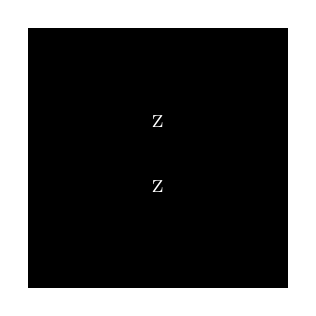
\begin{tikzpicture}[x=1.1\dimensions, y=1.1\dimensions]%f10
\draw[draw=none, fill=black] (-1,-1) rectangle (1, 1);
\node[color=white] at (0,-0.2225) {\scriptsize \light};
\node[color=white] at (0,0.2775) {\scriptsize \light};
\end{tikzpicture}
\end{document}